\label{chap:linguistic_persuasion}

\section{\statusgreen Introduction}
\label{sec:lp_intro}

% what (orientation)
In this second experimental chapter, we introduce a new ingredient in our analysis: persuasion techniques.
With the previous Chapter~\ref{chap:common_ground_search}, we underlined our need to understand how different terms, that are used to describe the same details, can effectively convey a different message to the readers.
Therefore, in order to characterise those differences, this chapter introduces \gls{persuasion} as an umbrella term that encompasses several techniques where the writer of a piece of text is trying to persuade the reader of a certain point of view.
% In this chapter, we add our second ingredient: persuasion.\todoAW{abrupt start}
% We intend persuasion as a general umbrella that encompasses several techniques where the writer of a piece of text is trying to persuade the reader of a certain point of view.

% why (rationale)
From the last chapter~\ref{chap:common_ground_search}, 
%we concluded with the need to understand how specific terms are used to persuade the reader. 
we are able to extract terms that have been changed in related articles, from sentences that are very similar but have still some differences.
We want now to quantitatively analyse these detected variations to quantify their specific use of persuasion techniques.
% \todoHA{Why? What is the value of this detection?}
In this way, we can understand if the specific term choices are in fact done to persuade the reader of a specific idea, or if they are only the manifestation of random choices.

For this reason, this chapter investigates the \emph{linguistic techniques of persuasion}, in other words, how the persuasion manifests itself on the linguistical surface.

% aim
Our motivation is to analyse whether the terms that change between multiple articles/sentences are correlated with the linguistic techniques of persuasion.

The Research Questions we want to answer are: 
\begin{enumerate}
    \item \emph{What do writers use to persuade the reader?}
    \item \emph{How can we automatically detect those techniques [which are used by writers to persuade]?} % Which are the possible indicators of these differences? // 
    \item \emph{How are the differences between similar articles} (extracted in the previous chapter) \emph{related to a different use of persuasion techniques?} % Is there a link between the parts that are different and persuasion techniques (propaganda/loaded language)? // 
    \item If the same story can be narrated differently depending on the persuasion techniques used, then persuasion is adding variations to the narration. Therefore, \emph{how much of an obstacle is persuasion in recognising the events in multiple articles?} %(clustering)
    %\todoHA{What led to this RQ? Previous text does not lead to this}
\end{enumerate}


% method
% strong/loaded language: using sentiment analysis tools 
% 18 techniques of propaganda

% Experiment together with common ground search
To answer these research questions, we take from Chapter~\ref{sec:lit_persuasion} the most commonly/recently analysed \gls{persuasion} means for which we have computational detection methods: \gls{propaganda} and \gls{sentiment}.
%\todoHA{Any refs that link propaganda and sentiment with persuasion?}
\todoAW{Harith asks what links propaganda, sentiment and persuasion. I'd ask what separates them. ie. why do you need to study persuasion at all if you can detect the other two cases?}

% BEGIN response to HA
As discussed in Chapter~\ref{sec:lit_persuasion}, we consider here \gls{persuasion} as a term that encompasses both \gls{sentiment} and \gls{propaganda}. % and populism
It is linked with sentiment because of its goal to influence the emotional response~\citep{gatti2014sentiment,rocklage2018persuasion,petty2015emotion,desteno2004discrete}.
And the relationship with propaganda comes from the inherent goal of propaganda to influence the view of the public about an idea or a group~\citep{bernays,jowett2018propaganda}.

% It is known that persuasion is related to an emotional response from the reader/listener, being related to emotions.
% Persuasion and Discursive Repertories~\cite{orrumachine}
% propaganda is a``consistent, enduring effort to create or shape events to influence the relations of the public to an enterprise, idea or group''~\cite{bernays}.
% Persuasion and Propaganda: ~\cite{jowett2018propaganda}.
%, populism.
% END response to HA


% carry the following experiment:
Therefore, we have the first part of this chapter that covers the detection of these persuasion techniques (Section~\ref{sec:lp_techniques}).
And then, we put this in relationship with the analysis from the previous Chapter~\ref{chap:common_ground_search} in Section~\ref{sec:lit_relationships}.
In this last part, 
we take into study the terms that change between articles, and we analyse whether they contain some persuasion techniques, and in which relationship. %indicate something about the changes in the sentences.

This is implemented according to the following pipeline:\todoHA{Rationale?}
\begin{enumerate}
    \item Analysis from Chapter~\ref{chap:common_ground_search}: extracts the words that are changed between similar sentences of similar articles
    \item Extraction of different techniques (sentiment, propaganda) on the sentences (described in the next Section~\ref{sec:lp_techniques})\todoAW{Doesn't your earlier paragraph suggest that we've already got this? ("means for which we have computational detection methods: propaganda and sentiment"))}
    \item Analysis of the relationship between these techniques and the changes in the sentences (described in Section~\ref{sec:lp_relationship})
\end{enumerate}


% findings
We discover that
the initial methods for fine-grained propaganda detection seem to be more promising %\todoHA{How? In what way?}
than sentiment detection.
Fine-grained propaganda analysis gives a multidimensional result because it provides the amount and words for each specific technique. Instead, sentiment only provides a mono- (or bi-) dimensional result. And furthermore, it shows weaker results, as will be shown in the next sections.
Sentiment is (cor)related to the specific propaganda technique of \texttt{Loaded\_language}, and having one technique instead of $18$ is only a disadvantage.
% does not provide useful insights when observed together with the changes occurring in the articles. 
The multi-dimensionality of propaganda across the techniques is much more useful.
For this reason, we mainly use propaganda for the experiments of the following chapters. 

Our findings from this chapter include:
\begin{enumerate}
    \item The relationship between the changed terms and propaganda language is not very clear: different parts do not always contain loaded language or propaganda. A lot of changes are not meaningful in terms of propaganda: linguistic variance.\todoAW{Not sure what you're getting at here.}
    \item As we hypothesised, the persuasion in the articles is adding terms and concepts that create variations (fitting different persuasion goals). As a consequence, these selected words make it slightly more difficult to recognise groups of articles related to the same event.
    Removing propaganda and/or sentiment from articles makes related articles slightly easier to cluster correctly.\todoAW{Not sure what you mean by this. In most cases of cluster analysis, there's no meaningful concept of a "correct cluster"}
    %\todoHA{For what? Not discussed earlier}
\end{enumerate}

% interpretation

% TODO: Interpretation? Or just pointers to next sections
The next sections are organised as follows. Section~\ref{sec:lp_techniques} contains some techniques that we identifed being related to persuasion.\todoAW{? I don't know what you mean by "related to" here.}
We present there what they are able to detect on our datasets (stage 2 of the pipeline above described). Then Section~\ref{sec:lp_relationship} contains two experiments aimed at understanding the relationship between these techniques and the words changed (stage 3 of the pipeline).

\section{Different Techniques of Persuasion}
\label{sec:lp_techniques}

% TODO preamble to different techniques: sentiment, propaganda, populism, ...

From all the different methods and approaches described in Chapter~\ref{sec:lit_propaganda}\tododefault{check ref}, in this section, we are using a set of methods to detect phenomena related to persuasion. % and do that at the word-level.
In other words, we are detecting several techniques that we know 
%\todoHA{Assume? No references to support this assumption} 
to be related to persuasion~\cite{gass2018persuasion}: sentiment and 18 different propaganda techniques.% and populism.
%\todoAW{I imagine that there's probably quite a lot of linguistics literature in this area that you should look at, if only to pin down your terminology. → easier to work out the terminology. At the moment I have persuasion (as top) then prop/sentiment/ that are subclasses. Look in literature.}

When selecting which techniques to target, we have an important requirement to keep in mind: we are interested to work at the word-level, because our end goal is to study how persuasion techniques relate to the variations across the articles (as will be seen in Section~\ref{sec:lp_relationship}). Only having a score for the whole article or for a whole sentence is not helpful, because we need word-level information.\todoAW{Not sure what you're getting at here. What information exactly are you hoping for at the word level? And it's not usually single words that persuage; rather, it's usually a sentence or article. So it's fine to want to identify the properties of the words that make them propagandistic, but I'd be wary of suggesting that that means you shouldn't be trying to also do a sentence- or article-level analysis.}
We are analysing word substitutions.

In the following subsections, we illustrate the models that we are using to perform sentiment detection (Subsection~\ref{ssec:lp_techniques_sentiment}) and fine-grained propaganda detection (Subsection~\ref{ssec:lp_techniques_propaganda}).
Then in Subsection~\ref{ssec:lp_techniques_populism_vs_propaganda} we show some work done on populism. Even though we don't have computational detection of populism, we wanted to see the relationship that it has with propaganda.\todoAW{Not sure this para is necessary}

\subsection{\statusorange Sentiment detection}
\label{ssec:lp_techniques_sentiment}

First of all, we start with some sentiment detection. It is known that persuasion is very often related to an emotional response from the reader/listener, being related to emotions~\citep{rocklage2018persuasion,petty2015emotion,desteno2004discrete} and to sentiment~\citep{gatti2014sentiment}.
While computational approaches to detect emotions exist (usually quantified across the 5-big emotions), the computational tools available for sentiment detection are more numerous and more common. The main disadvantage of only using sentiment detection instead of emotions is that it usually gives an output on 1 or 2 axes:\todoAW{Wouldn't a 2-dimensional analysis be more fine grained than a 5-bucket "big emotion" analysis? In which case, it's an advantage of using sentiment rather than emotions.}
valence (positive or negative) and strength (from neutral to strong). But for an initial analysis, we deem\todoAW{How?} that sentiment is enough.

For detecting the sentiment, we decide to use term-based analyses that, despite being less accurate than huge deep-learning models, %\todoHA{in comparison to what?}
they can provide the specific words responsible for the output. We need to see which words are responsible for the sentiment scores, so we are accepting less accuracy if necessary.\todoHA{unclear} Our main reason is to be able to find words that are loaded with sentiment. If the score of sentiment is not perfect, it is not a problem.\todoHA{unclear} \todoHAinline{You are telling the reader that accuracy will be bad, and that this is ok. But unclear why it will be bad, and why this is ok. Better to leave accuracy to much later, rather that accepting low accuracy upfront}
In the next subsections, first we describe the chosen detection tools, then we describe how we combined them together, what they are able to extract on our datasets. Finally, we conclude with some findings that we discovered while applying sentiment detection to news articles (big variations of sentiment across the articles, correlation with quotation).
\todoAW{If you're using OTS sentiment analysers, you don't really need to justify their lack of accuracy. Rather, you should focus on what it means for your own results, and whether the (lack of) performance of the sentiment analyser will excessively impact your work.}

\subsubsection{\statusgreen Sentiment analysis tools}

For detection, most of the methods that we pick are lexicon-based. This happens because of our focus on getting the words responsible for the scores.\todoHAinline{change the order. start by explaining your needs, and justify them, then explain what you found/selected} Most of these tools work based on a lexicon that is combined with different scoring mechanisms (e.g., sentistrength, textblob, vader). They are built around a lexicon where each word has a specific score, and some combination rules. But we do not exclude tools that work with a different, more complex approach. It is only required from them to give a score specific to the individual words. For example we use Stanford CoreNLP which is based on a RNN~\citep{socher2013recursive} that accounts for the sequence but also for the dependency tree of the sentence (in other words, discovering the combination rules autonomously). It is not based on a lexicon, but instead on a more complex dataset linking sentiment scores to a dependency tree.
% We selected the following methods: sentistrength, textblob, vader, Stanford CoreNLP

% Describe each of the methods
Here we describe each of the methods used.

\paragraph{Sentistrength}
The first tool considered is Sentistrength\footnote{\url{http://sentistrength.wlv.ac.uk/}}. This tool is built around a lexicon of 2546 words (or in some cases \emph{word stems}) where each entry is annotated with a score (integer in the range $[-5;5]$) and a set of combination rules considering negations, boosters, questions. The outputs given can be retrieved in different forms:
\begin{itemize}
    \item Dual score: as the name suggests, it gives two values, one for the Negative score ( -1 not negative to -5 extremely negative) and a Positive score (1 not positive to 5 extremely positive). A sentence can be both positive and negative so the two scores are independent
    \item Binary $\set{positive, negative}$
    \item ternary $\set{positive, neutral, negative}$
    \item Scale: integer value in $[-4;4]$,
\end{itemize}

But, as we said, we are interested in the single words responsible for the sores, so we needed to adapt the tool to output them. We achieve this by comparing the sentences with the lexicon and outputting the original scores given to them.


\paragraph{Vader}
Very similarly to Sentistrength, also Vader\footnote{\url{https://github.com/cjhutto/vaderSentiment}} has a lexicon-based approach and does not natively give in the outputs the words responsible for the sentiment. Vader has been built mostly to analyse social media content, optimised for short texts.
Its lexicon is composed of 7520 words with each entry has the raw annotations (10 annotations with integer value in $[-3;3]$) and the mean score + standard deviation.
The outputs can be read in two modalities:
\begin{enumerate}
    \item compound: where each analysed text gets assigned a single value (float) in the interval $[-1;1]$ (-1.0 negative 0 neutral 1.0 positive)
    \item separate scores: Positive, negative and neutral scores which sum to $1.0$
\end{enumerate}

Also for Vader, to obtain the single words that are loaded with sentiment, we take a look at the lexicon to match manually. The advantage of this tool is that the lexicon is much larger than the one from Sentistrength.
\todoAW{Risky comment: you can modify sentistrength with your own lexicon and then retrain it. This is pretty well established, so I don't think you can really count this as an advantage unless you can convicingly argue that you've a good reason for only considering the prebuilt models.}



\paragraph{TextBlob}
The next tool is TextBlob\footnote{\url{ https://textblob.readthedocs.io/}}, which instead provides the words/parts responsible for the sentiment natively.\todoAW{?}
The lexicon only contains adjectives, in total 2918. Each one of them is marked with the \emph{polarity}, \emph{subjectivity}, \emph{intensity} (for the booster words)\todoAW{What's a booster word? "very", for example? If so, that's an adverb, not an adjective.} and with the \emph{confidence}. Having these scores, the tool keeps track of the input text across two dimensions: polarity and subjectivity.
Therefore, the outputs of the analysis are the two scores of \emph{polarity}, a real value in $[-1;1]$ (-1 negative, 0 neutral, 1 positive), and \emph{subjectivity}, a real value in $[0;1]$ (0 objective, 1 subjective).

Relatively small lexicon, but it has the advantage of being focused on the adjectives.\todoAW{Why is that an advantage? If I describe someone as a "bearded idiot" for example, then I'm intending the noun to be the main sentiment bearer rather than the adjective.}
Combining it with the other tools enables us to expand the overall lexicon.


\paragraph{Stanford CoreNLP}
Finally, Stanford CoreNLP, which is a tool that performs several NLP tasks, and one of them is sentiment analysis.\todoAW{verb? Sentences, please!}
The sentiment detection, differently from the previous tools presented here, is based on a more elaborated approach involving a special RNN which relates to the parse tree. 
The dataset used to train this sentiment analysis model is Sentiment Treebank\footnote{\url{https://nlp.stanford.edu/sentiment/treebank.html}} which contains sentiment scores linked to dependency trees).
The outputs of the sentiment analysis module are dual. There is an overall score of sentiment to the full sentences. And also it generates a SentimentTree which is a representation of how the sentiment is conveyed from the leaves (the single words) to the full sentence, following the dependency tree.
The scores in output (both total and parts of the tree) have an integer value in the interval $[0;4]$ (0 = Strong\_Negative, 1 = Weak\_Negative, 2 = Neutral, 3 = Weak\_Positive, 4 = Strong\_Positive).

From the SentimentTree, we wrote a parser\todoAW{I don't think we did; writing a parser is a major undertaking.} that parses its syntax and extracts the scores to the single words.\footnote{\url{https://github.com/MartinoMensio/corenlp-sentiment-tree-parser}}
In this way, we are able to see the sentiment of the single words and not only the overall score for a sentence.\todoAW{Really needs some examples to illustrate this point.}

\subsubsection{\statusgreen Combination of the tools}
\todoHAinline{deciding to combine upfront is not very good. Better way is to use them individually, then combine. This way you scientifically demonstrate value of each approach.}
% Why combine
From this list of tools, we decided to combine them together in order to increase the rate of words detected as sentiment-carrying.\todoAW{I think you mean that you wanted to improve the accuracy of the sentiment recognition.}
As each one of them has different\todoHA{what if they contradict each others?} lexicons covering different groups of words (e.g., TextBlob only adjectives), and given that they do not overlap totally,\todoHA{avoid such vague language. This is also not supported by any data. Why not?} the combined lexicon (not correct word, because CoreNLP does not use one) / detection power can be much larger than just considering one of them.

% How combined all of them
We therefore combine them in the following way:
\begin{enumerate}
    \item running the tools in parallel;
    \item collecting the results;
    \item numerical scores: uniforming the scales (each tool has a different one) and averaging the single scores out;
    \item sentiment words: doing the union of the words outputted by each tool, and for each word computing the average score (again by uniforming the values first).
\end{enumerate}
% we run them in parallel for each input text, and then we collect the results.
% We consider two types of outputs: the score(s) given to the text, and the words responsible for the score.

% For the score, uniforming the scales and doing the average. Ranges --> conversion --> average

% For the words, we take the union of the words outputted from each tool. Each word can then have a positive/negative score so we also merge them,.
% If one word is given back by just one tool, then the score is given by the tool (uniforming again the score as above). Instead if the word is given back by multiple tools, we consider it only once and we average the uniformed scores.

Even if we average and combine the results, we keep the original outputs for each tool in order to backtrack the results and see where the problems come from.

To uniform the scales, we consider two main axes: polarity (used by all of the tools) and strength (provided by SentiStrength, and subjectivity by TextBlob). We map the numerical intervals from $[min;max]$ to $[-1;1]$ by means of a linear transformation. The categorical values, instead, are mapped by firstly sorting the output labels from negative to positive, then converting to increasing numerical values (e.g., for 4 labels, $\set{1,2,3,4}$) and then applying the linear transformation as in the other case.
\todoAW{Would it have made more sense to combine the lexicons from the different systems and then used them to augment one of the existing models (eg. SentiStrength)? Even if not, you should be prepared to answer that question in your viva.}

\subsubsection{\statusred Statistics over our datasets}

\todo{stats over our datasets}
% How they perform separately on the dataset (justifying why all of them) and the result of combination.
In this subsection we provide some statistics about how the described approach for sentiment detection works on the datasets we selected.

% Datasets: AllSides, AllNews
First of all, as described also in the previous chapter, we rely here on two datasets: AllSides and AllNews.

The first one, AllSides, contains X \todo{copy main numbers from chapter 3}

The second one, AllNews, ...\todo{finish}

% average scores
Scores:
- Unified scores by each tool (polarity and strength)
- Correlation between tools

Words:
- percentage of words detected by each tool
- percentage of words detected by combination
- term analysis: most frequent words positive/negative

Group by News source:
- sources with highest/lowest/strongest
- most frequent sentiment words for the most frequent sources

$\rightarrow$ good fit for a figure by news source\todo{figure by news source}

Problems of the tools: 
- false sentiment words. How am I compensating for it?

Combined results


\subsubsection{\statusorange Sentiment variation along articles}

With this setup of the tools, we moved to inspect the articles more closely. We want to see how the sentiment evolves inside a single article\todoHA{unclear} and if it is linked to any other external factors.\todoHA{like what?}\todoAW{Such as the reader? Very vague!}
% We then experimented with the selected libraries to see how they could analyse the sentences in news articles. 
We started by observing how the sentiment scores vary across one article at a time, when we consider the sentences of the articles.\todoAW{Earlier, you were arguing that you were concerned about word-level sentiment rather than the sentence or article level}
For each sentence, we compute the sentiment scores and then we compare how the tone changes across a single article at a time.\todoHAinline{changes how? and what change would tell us? remember that reader won't know why you are doing something unless you make that clear}

Figure~\ref{fig:sentiment_across_one_article} shows how the detected sentiment changes a lot across an article.
\todo{which article is it? Why this one?}
Some sentences appear to be very neutral, and some instead are very subjective/intense.

\begin{figure}[!htbp]
    \centering
    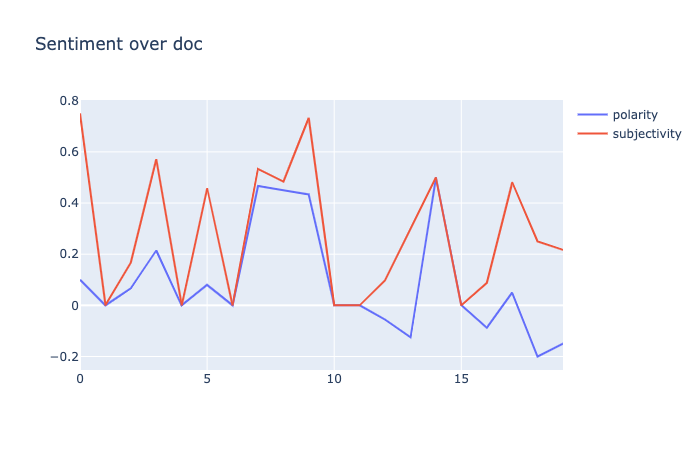
\includegraphics[width=\linewidth]{figures/sentiment_across_article.png}
    \caption{Sentiment along a single article. Each point on the x axis is a different sentence, while vertically on the y axis several scores are plotted.}
    \label{fig:sentiment_across_one_article}
\end{figure}
\todoAW{I don't understand this. Why aren't the axes labelled? What does the title mean? And where is the graph described and interpreted in the text?}
\todo{Fig~\ref{fig:sentiment_across_one_article} coming from which libraries?}

% \subsubsection{Sentiment is correlated to quotation}
By looking closely at several articles where this behaviour\todoAW{What behaviour?} occurs, we noticed that this duality of tones\todoHA{clarity} in the articles is mostly correlated to direct/indirect reporting. When the articles give space to some interviewee (quoted)\todoHA{shouldn't this be part of the evaluation? why mentioned here?} the sentiment libraries detect intense and subjective words/scores. Instead, when the reporter is narrating, the tone is quieter and more neutral.
\todoHAinline{you need examples throughout}

To study this correlation on large scale on our dataset, we tested our observation\todoAW{Do you mean that from the observations you formed a hypothesis, which you then tested?} by automating it.
On one side, using the sentiment libraries. On the other, using a model for quotation detection~\citep{scheible2016model}.\footnote{\url{https://github.com/christianscheible/qsample}}\todoAW{Sentences!}

For each sentence, we computed both sentiment score and the quotation percentage (defined as number of words inside a quotation divided by total number of words).
Figure~\ref{fig:sentiment_vs_quotation} shows for the same example article, how the two measures are moving together.

\begin{figure}[!htbp]
    \centering
    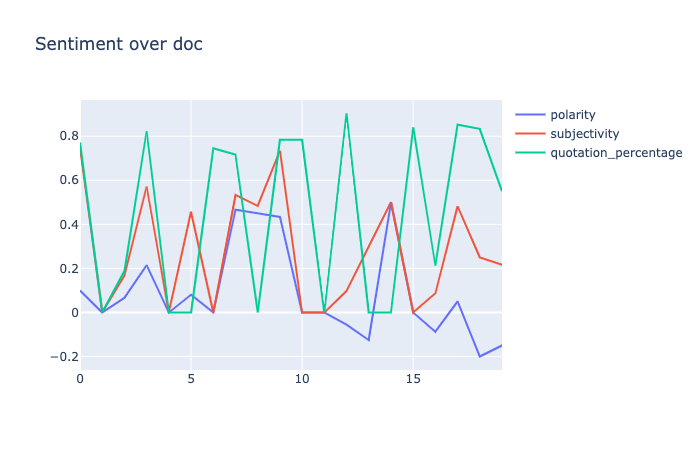
\includegraphics[width=\linewidth]{figures/sentiment_vs_quotation.png}
    \caption{Sentiment VS quotation}
    \label{fig:sentiment_vs_quotation}
\end{figure}
\todoHA{This is too crude. Think of a more precise way of measuring such correlations}

\todo{correlation stats across all the dataset? Quantify. Total correlation across the dataset: ??}

Findings recap

Finding 1:
Subjectivity and quotations: quotations increase subjectivity of articles, are the most subjective parts

Finding 2 (shown in previous subsection): the results of lexicon-based sentiment detection are not very great, and they are prone to many errors.

\todoHAinline{What is the conclusion here?}

\subsection{\statusorange Fine-grained Propaganda Analysis}
\label{ssec:lp_techniques_propaganda}

As a second group of persuasion techniques, we consider \gls{propaganda}.

Propaganda is a form of persuasion that is characterised by its goal to indoctrinate population towards an individual or a particular agenda.\todoAW{Find a good quote from the political discourse literature if you can.}
It manifests through several techniques that have been studied in the literature. Each technique has its own peculiarities.

For detecting propaganda, we want an approach that gives us not only a binary label (propaganda vs non-propaganda), but we want to have an insight about which specific techniques have been used. For this reason, we need to have fine-grained detection of propaganda, that produces as output the specific techniques used and which words are responsible for it.
Taking from the literature described in~\ref{sec:lit_propaganda}, we consider the recent work of~\cite{da2019fine} as it is the only one\todoHA{Too strong} that has fine-grained detection. This method uses a neural network to annotate text articles and to see which words belong to specific propaganda techniques (Figure~\ref{fig:propaganda_example_1}).
The model is a sequence model based on BERT. It is based on the dataset~\citet{TODO} which contains articles annotated at the span level (specific words are highlighted and assigned to a specific technique). The model then learns to reproduce these annotations by looking at words in their context (sequence model).

It performs classification on the word level. Each word is classified as being one of 18 different techniques or none of them.

From its publication paper~\cite{da2019fine}, we can see in table 6 and 7 that this model has been evaluated in two ways:\todoAW{Did you attempt to reproduce this evaluation?}

\begin{itemize}
    \item sentence-level: binary classification, whether the sentence contains propaganda or not. For this task the reported F1 is around $60\%$\todoHA{reported dataset? clarify}
    \item span-level (full task): whether the corrects words\todoHA{?} have been identified with the correct technique or not, so accounting both for position/boundaries and for the label. For this task the reported F1 is slightly above $22.5\%$
\end{itemize}

These statistics make us aware that, even though this model is the currrent State of the Art, its ability to recognise the proper techniques of propaganda are quite low overall.
Therefore we need to take with a grain of salt the outputs coming from this model.\todoAW{Too informal. What does "tak[ing something] with a grain of salt" mean in practical terms?}

\todoHAinline{leave self-criticism to later. also, reported \% here are only indicators since other data is different to yours}

\subsubsection{\statusred Statistics over our datasets}
\todo{Here talk about general setup, statistics of applying propaganda detection over news articles in our datasets.}

Datasets

Stats: definition of word-based percentage, overall word-based percentage of propaganda (any techniques), technique specific percentages. Term analysis: most frequent across techniques, technique-specific terms


\subsection{\statusgreen Propaganda vs Populism}
\label{ssec:lp_techniques_populism_vs_propaganda}

% from "Propaganda datasets unbalanced?"
% What
In this section, we experiment with another concept from the literature that is shown to be close to persuasion and propaganda: \gls{populism}~\citep{tumber2021routledge,pasquino2008populism}.\todoHA{Not mentioned in intro. Why not?}
We want to understand: is there\todoHA{?} is any substantial difference between populism and propaganda?
This question arises purely from a logistical point of view: we have automated methods for detecting propaganda, but we do not have tools to detect populism. Therefore, if we can prove that populism and propaganda are actually correlated, then it becomes not important for us to be able to detect something that is very much correlated to something else that we already detect.

% concepts
On the conceptual level, propaganda and populism are two separate concepts. The first describes more the persuasion mean used to push for an agenda, while the second one is usually used more together with the actor that wants to push the agenda. Populism is ``a type of politics that claims to represent the opinions and wishes of ordinary people".\footnote{\url{https://www.oxfordlearnersdictionaries.com/definition/english/populism}}
And to be on the side of ordinary people, it uses propaganda as a mean. So a populistic \emph{actor} uses propaganda \emph{techniques}. Conceptually, they are related.

\todoHAinline{ok, but what would detecting populism give you? Why is this of value?}

\todoHAinline{I would start by: 1. explaining value of detecting populism. 2. detecting it and evaluating that, then 3. see if correlated with propaganda}

% practically/computationally
On the computational/detection side, we want to see if this relationship between populism and propaganda stands.
So to evaluate it, we have computational approaches for propaganda detection, but not for populism detection.
A solution to this problem, is to use a dataset where we have the ground truth for the populism, which will be run through the propaganda detection pipeline. Then we will compute the correlation between the two, and we can establish whether this relationship is proven. The advantage of using directly the ground truth for one of the two phenomena (populism) is that we can only have errors for the propaganda detection.\todoHA{unclear} Instead, if we were to compare two predictions, the errors could be on both sides.

% dataset used
For this experiment, after looking at the available datasets for populism, we selected the one from~\citet{hawkins2019global} because it is quite balanced in terms of the political orientation of the actors annotated (liberal vs conservative).\todoAW{It strikes me here that this is a very US-centric interpretation of the political landscape. Do you consider whether the make up of the dataset poses any threats to validity?}
It contains 1240 political speeches, from several countries and languages
For each one of them there are four annotators that give a numerical score of populism in the range $[0;2]$ where $0$ means non-populistic and $2$ means very populistic. The single annotations are already averaged out.
So from the 4961 raw rows, by deduplicating (4 annotations for each speech) we have 1240 speeches, out of which 265 are in English (then down in the rankings, 304 in Spanish and 148 in Portuguese).

% These 265 speeches all have a leaning classification (we will see more about leanings in the next chapter): 36 left, 37 center, 84 right, 106 NA. We use this information in order to check whether the results that we get are general across the political spectrum.
% --> moved to chapter 5


% Dataset found: populism in political speeches %https://dataverse.harvard.edu/dataset.xhtml?persistentId=doi:10.7910/DVN/LFTQEZ&version=2.0 
% Each annotator (4 for each speech) gave a score between 0 (non-populistic) to 2 (very populistic)
% 4961 rows 
% 1240 deduped (352 left, 256 center, 469 right, 652 NA)
% Languages: 265 en (304 es, 148 pt, …),
% Leaning of the english ones: (36 left, 37 center, 84 right, 106 NA)



% Goals:
With this dataset, as we described, we want to compute the 
correlation between propaganda and populism. So we take each speech in the corpus and we proceed to compute the Spearman's correlation~\citep{spearman1910correlation} between the  populism averaged out between the annotators and different propaganda metrics: total word-based percentage of propaganda, and word-based percentage of each of the propaganda techniques. 


% results
The Spearman's correlation between the populism and the total word-based percentage (all techniques together) is $0.1694$. This value is quite low. So it seems that they are quite unrelated.\todoAW{This feels to me like the sort of investigation and analysis which forms the bedrock of your research. So I think you need to set it out more formally so that it feels like less of an aside.}

\begin{figure}[!htbp]
    \centering
    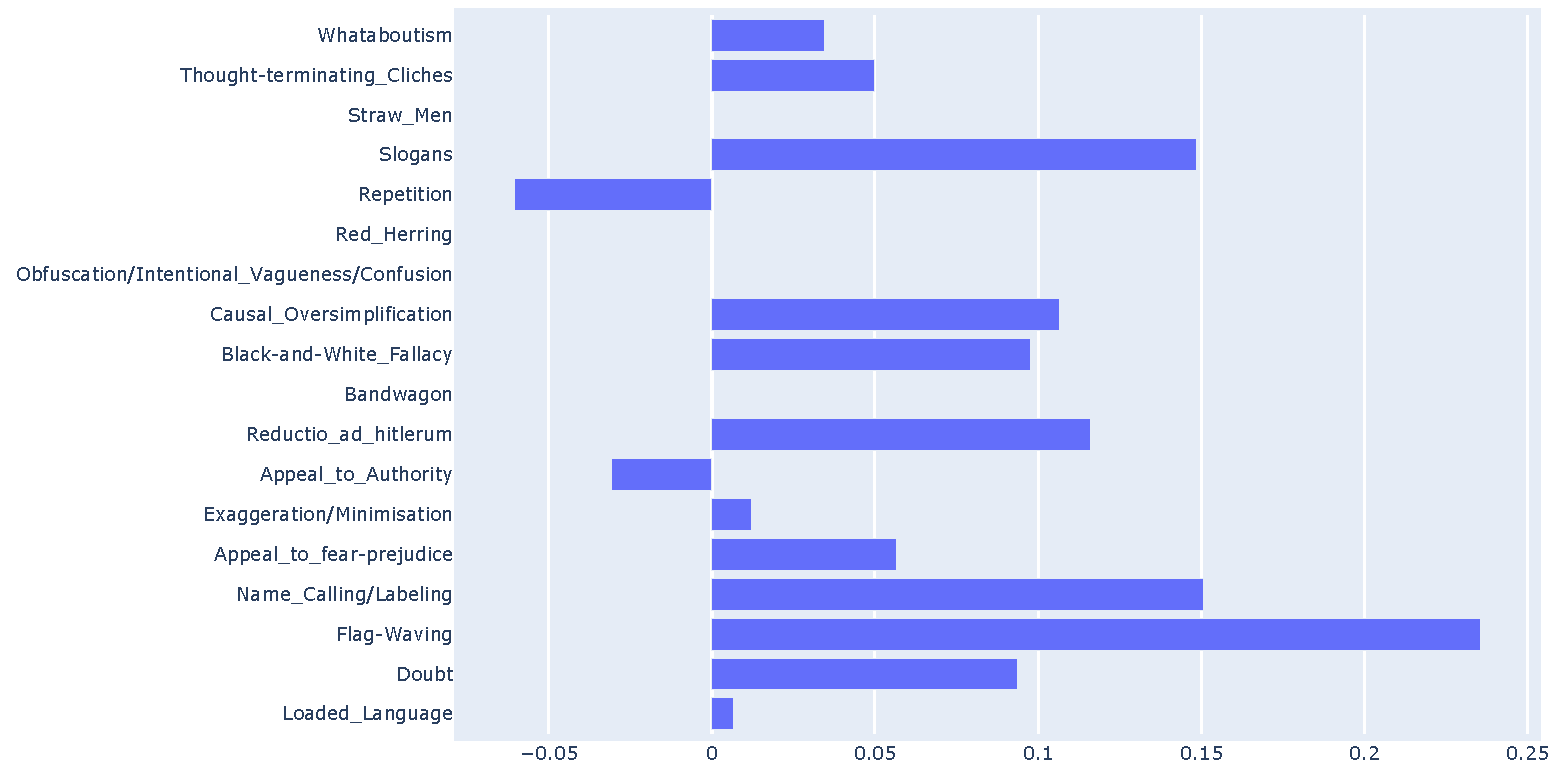
\includegraphics[width=\linewidth]{figures/populism_propaganda_correlation.pdf}
    \caption{Spearman's correlation between populism and each propaganda technique}
    \label{fig:populism_propaganda_correlation}
\end{figure}

By breaking it down to the correlation of populism to each propaganda technique, we can see in Figure~\ref{fig:populism_propaganda_correlation} that the strongest correlation is found with \texttt{Flag-waving}, \texttt{Name\_Calling/Labeling} and \texttt{Slogans}. Some of the techniques have very low correlation. It is interesting to notice that two techniques have slightly negative correlation (\texttt{Repetition} and \texttt{Appeal\_to\_Authority}), so this means that they are used by less populistic speeches.


% L/R evaluation:
% Assumption: propaganda correlates to populism similarly in L/C/R
% Result total: 0.225 Left, 0.005 Center, 0.374 Right → Why? Is it a matter of quantity of populism/propaganda?
% Populism average:  [0.1259, 0.0729, 0.2712]
% Propaganda average: [0.0165, 0.0271, 0.0432]
% Ratio: [0.1317, 0.3717, 0.1593] → populism over propaganda ratio is a bit bigger on right (21\% more), but the correlation Right is bigger than left of 66\%. So it is less likely that this is just a matter of quantity. On the Right, propaganda and populism are strongly linked

% findings
Propaganda and populism are correlated, but not too strongly.\todoAW{?}
The fact that some of the techniques are correlated to populism is a good sign,\todoHA{why?} even though the correlation scores are still low to be considered as ``strong ccorrelation''. We will expand this experiment in the next Chapter when we take into consideration political leaning.
Considering that the current fine-grained propaganda detection is not so accurate (cf. Section~\ref{ssec:lp_techniques_propaganda}), we can say that this weak correlation can still be considered as a signal that the two phenomena are related.
% In the Right more. This is one point supporting the hypothesis that propaganda detection works better in the Right than in the Left. → unbalanced detection caused by unbalanced data



\section{Relationship between techniques and words changed}
\label{sec:lp_relationship}

After having described in the previous sections the detection of the \emph{linguistic techniques of persuasion} on their own, we describe in this section the last stage of the pipeline announced in the introduction to this chapter (Section~\ref{sec:lp_intro}).

Therefore, here we analyse the relationship between the linguistic techniques of persuasion, and the variations across the articles (from previous Chapter~\ref{chap:common_ground_search}).

To analyse this relationship, we have two different experiments:

\begin{enumerate}
    \item small variations vs detected persuasion: we want to investigate if the small variations (between several texts about the same event detail) can also be seen with changes on the detected persuasion; \todoHA{unclear}
    \item removing persuasion to improve clustering: is persuasion acting as noise when we want to cluster news articles? We want to test what happens when we remove persuasive words from the articles.\todoHA{why assuming it might be noise?}
\end{enumerate}

\subsection{\statusorange The effects of small variations on detected persuasion}
\label{ssec:lp_relationship_small_variations}

\todoAWinline{It all starts getting very choppy from here. In general, I think the main thing in this chapter is that your experiments need to be presented more formally. You have interesting looking results, but I don't really see where they come from.
Ask yourself how someone would reproduce the work you've presented here. I wouldn't know how to start.}


% Why
% What
For this experiment, we want to observe how the small changes detected in the previous chapter affect the detected persuasion.
Having computing methods for sentiment and for fine-grained propaganda detection, we decide not proceed with populism detection,\todoHA{probably move section on populism to the end since it is weak and experiment not thorough}\todoAW{I'm not entirely clear what that decision was based on.} but only keeping as axes for measurements the sentiment ones (strength and polarity) and the 18 propaganda techniques.

% RQ3
Our RQ3 is ``how are the differences between similar articles related to a different use of persuasion techniques?".
So to answer this question, here we take groups of linked sentences (from chapter 3) and we see how their variations are related to changes in persuasion.

\subsubsection{Dataset}
\label{ssec:lp_relationship_small_variations_data}

% data
For this experiment we use a set of pairs of sentences (extracted from the analysis of chapter~\ref{chap:common_ground_search}) which are characterised by high similarity score (\acrshort{use} model).

The dataset of origin is Google News Headlines, as it presents clusters of articles with a high number of articles each (between 20 and 90). Therefore, applying the methodology described in Section~\ref{sec:cgs_clustering_and_differences}, with quite strict thesholds on the distance between sentences, we can still produce in output many cliques of sentences. These cliques contain sentences that have minimal variations and we aim with this current experiment to understand if they are related to a different usage of persuasion.
% Google headlines: articles are grouped in clusters. Clusters have around 20-90 articles each. Each cluster belongs to a certain broader topic (UK, World, Business, Entertainment, Sports, Science, Health). Positive sides: very large. Negative side: the clusters change over time, they are created by ML (not human-curated)

The Google News Headlines that we selected are between 8th September and 14th October 2020, because that is the timespan during which this experiment was conducted. We could repeat the experimentation in other timespans.
We extracted from them a subset of 138 sentence pairs, by using the approach described in the previous Chapter~\ref{sec:cgs_clustering_and_differences}:
\begin{enumerate}
    \item cliques of sentences extracted using Hierarchical Agglomerative Clustering, to be able to cut the similarity threshold at any point.
    \item Distance threshold for the cliques: minimal similarity of $80\%$ and maximum similarity of $98\%$ according to the \acrshort{use} model. In this way we select sentences that are related to the same detail (discarding sentences that are too different), but at the same time we discard sentences that are almost identical and only differ by punctuation or reordering.
    \item Random selection of a small subset of sentence pairs. From each clique of sentences (containing 3 or more), only two sentences are selected in order to avoid having three-way comparisons (or even higher grade).
    %\item Manual annotation of whether the differences in the sentence pairs are making use of different persuasion or relate to a different opinion / point of view. This specific data is used for the experiments ``comparison with manual annotations" at the end of this Section~\ref{ssec:lp_relationship_small_variations_qual}
\end{enumerate}



\subsubsection{Approach}
\label{ssec:lp_relationship_small_variations_appr}

Having as goal to understand the relationship between small differences in multiple versions of the same detail and the use of persuasion techniques, in this experiment we combine two analyses:
\begin{enumerate}
    \item Fine-grained differences analysis from the previous Chapter~\ref{sec:cgs_clustering_and_differences}. We take from this analysis both the link between similar sentences and the indication of how many and which words have been changed and which one are kept the same.
    \item Persuasion analysis seen in the previous Section~\ref{sec:lp_techniques}: we extract sentiment and propaganda techniques from the sentences. This analysis provides scores and the specific words affected.
\end{enumerate}

The point of contact between these two analyses, is to see how the differences relate to persuasion. In other words, see how frequently a change in the wording is related to persuasion, which persuasion techniques change mostly between these sentence pairs, and which specific words are responsible for this relationship between differences and persuasion.

% How: method
We describe persuasion with the help of sentiment detection (as seen in section~\ref{ssec:lp_techniques_sentiment}) and fine-grained propaganda detection (section~\ref{ssec:lp_techniques_propaganda}).
The comparison is done in different ways:
\begin{enumerate}
    \item score: sentiment or propaganda scores. For example, one change in an adjective could result in more negative sentiment, or in more of a specific propaganda technique;
    \item words: the words changed could be the words that carry sentiment/propaganda. And instead of just hypothesising that the change in the words are responsible for a different score (point above), we have a direct indication that the words belong to a persuasion technique.
\end{enumerate}

\todo{Figure with example: uniqueness of words highlighted, corresponding plot with scores of the two sentences, and also persuasion words in the text (different colour?). Take from one of the three on my desktop (only pair, not clique), and create the display on streamlit/displacy}

% split between computational results and human judgement
We conduct the analysis following two main points of view:
\begin{enumerate}
    \item computational-only: we compute how much the differences in wording affect the scores and words of detected persuasion;
    \item soft-validation of computational results: we try to see how good the detected changes in persuasion are when we compare to human-generated labels.
\end{enumerate}

% While the first one is less prone to criticism, being computed, the second one is less valid because only I annotated the sentences
The output measures are: on average, how many variations in percentage also imply a different measured persuasion (in terms of scores)? %Are the variations between the texts making the persuasion scores change? 
And, are the words changed also loaded with techniques of persuasion? 

% Results
The results have a first quantitative side and then also a qualitative one. ? rename to automated vs manual???
% it depends on which persuasion technique is considered.

\subsubsection{Computational results}
\label{ssec:lp_relationship_small_variations_quant}

\todo{compute metrics from results
Quantitative results\\
- reduce groups to pairs: select rows and merge\\
- count statistics about dataset: number of pairs\\
- find example and create figure with sentence pairs with scores, words\\
- add propaganda features (score and words) to each csv and merge sentiment analysis (score and words)\\
- compute score results: score changes average for each technique (shows which techniques are mostly affected by variations)\\
- compute words results: \#words persuasion / \#words changed\\
- plot results (techniques vs percentages)
}
% quantitative
Firstly, we computed some statistics over our dataset.
With the selected 138 samples, we have on average $32.0\%$ of the words that are unique in sentence pairs. The words that count as unique in a sentence pair are the ones that do not appear in the other sentence belonging to the same pair. This corresponds in our example of Figure~\ref{fig:TODO} to the words highlighted in green.

In the sentence pairs, the average percentage of words that are detected as related to any persuasion technique is $14.8\%$. Of these, most of them are detected as carrying sentiment ($12.5\%$) while only $3.2\%$ related to propaganda.

\begin{figure}[!htbp]
    \centering
    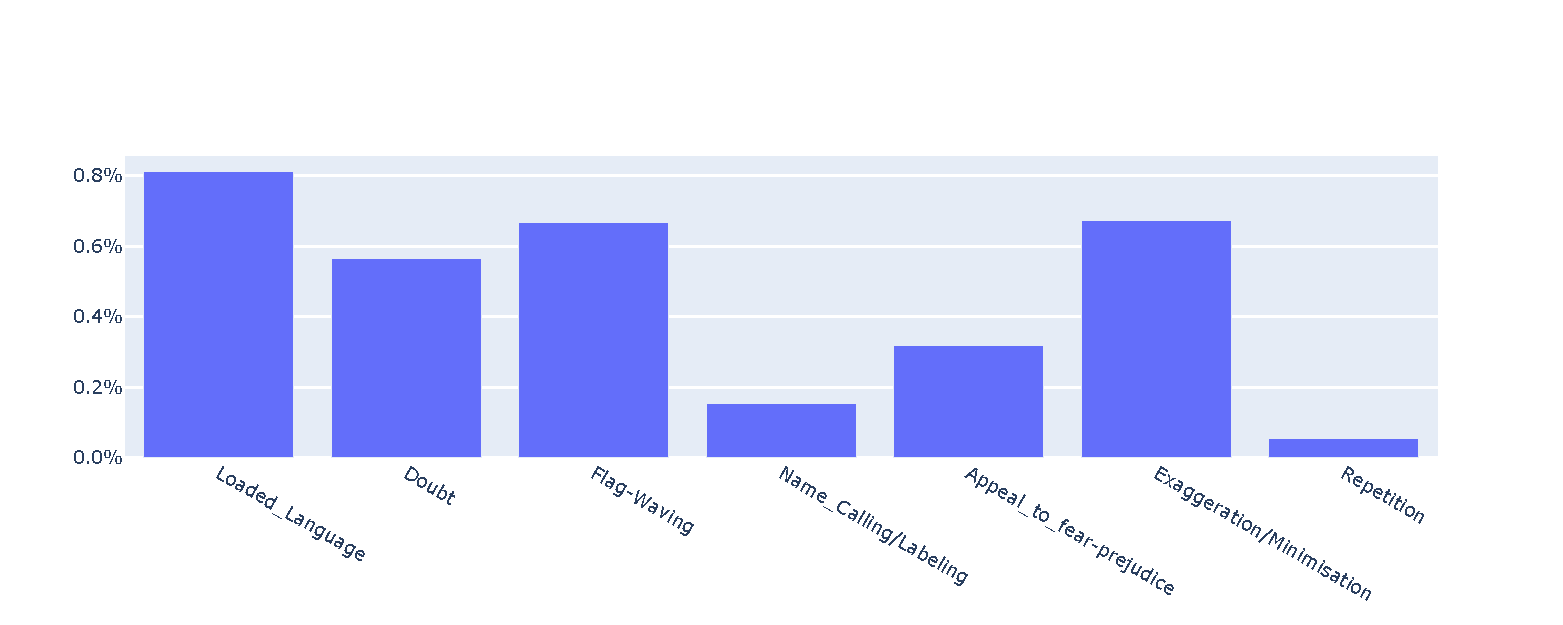
\includegraphics[width=\linewidth]{figures/4.3.1_propaganda_avg.pdf}
    \caption{Average of the detected propaganda techniques across the dataset of sentence pairs.}
    \label{fig:propaganda_avg}
\end{figure}

Figure~\ref{fig:propaganda_avg} shows the percentages of each detected propaganda technique in the corpus. We can see that the percentages are much smaller than the value provided by the sentiment libraries.
By inspecting the samples, we see that generally sentiment detection provides way more terms in result than the propaganda detection. This means that potentially more words are being recalled, but the precision is much lower because we see lots of false positives.

% number of changes vs score variations
Up to this point, the persuasion statistics were given on single sentences. This next paragraphs instead contain the analysis of the change of detected persuasion between the sentence pairs.
How many times the variation of the sentences results in a change over the persuasion scores? And how big is the change in the scores?
We answer these question by first considering every minimal change in the scores. And then by considering the magnitude of the change.


\begin{table}[!htbp]
    \centering
    \begin{tabular}{r|rr}
         Technique & any change & magnitude \\
         \hline
         any & 98.5\% & 0.0\% \\
        sentiment\_total & 98.5\% & 9.3\% \\
        propaganda\_any & 14.4\% & 3.4\% \\
        PROPAGANDA:Loaded\_Language & 7.2\% & 1.0\% \\
        PROPAGANDA:Doubt & 1.4\% & 1.1\% \\
        PROPAGANDA:Flag-Waving & 1.4\% & 0.4\% \\
        PROPAGANDA:Name\_Calling/Labeling & 1.4\% & 0.1\% \\
        PROPAGANDA:Appeal\_to\_fear-prejudice & 2.8\% & 0.6\% \\
        PROPAGANDA:Exaggeration/Minimisation & 1.4\% & 0.1\% \\
        PROPAGANDA:Repetition & 1.4\% & 0.1\% \\
    \end{tabular}
    \caption{Caption}
    \label{tab:change_scores_persuasion_in_variations}
\end{table}


The result of Table~\ref{tab:change_scores_persuasion_in_variations} show that in $98.5\%$ of the cases, we can see a change in the scores of at least one technique.
Breaking down this result, we have that in all these cases (still $98.5\%$) there is a change in the sentiment

Overall, on the quantitative side, we see that a portion (\%?) of the variations in the texts is causing a persuasion score change. Out of X couples of sentences with small variations, only for Y we see a change. Among these, Y1 are changes to the sentiment and Y2 to the propaganda score. The breakdown by techniques is illustrated in the blue bars of Figure~\ref{TODO}, which shows the percentages of variations that correspond to a change in the respective technique. (for each technique, for each sentence pair, a boolean yes/no where yes corresponds to ``changed" and no to ``unchanged", then counting the percentages of yes) 


%number of changes vs persuasion-loaded terms: how many terms in percentage?
And secondly, still on the quantitative side, we also compute a measure based on the words: how many changed words (percentage) are also persuasion related? To compute this, we have X words that have been changed (out of Z sentence pairs), and Y words that are related to persuasion.
With respect to the first measure, this metric is based on the words instead of being based on the number of samples. The red bars of Figure~\ref{TODO} illustrate it.\todoHA{Use tables to present results}

\todo{Barchart (horizontal) of: 1(blue) percentage of variations that also correspond to a change in the values for each of the techniques. X axis: percentage, Y axes: techniques. 2(red): percentage of words changed that also are persuasion related}

\todo{compute results: currently having a small problem with my pipeline, I need to put back together the articles used in the past from Google News. The dataset from AllSides instead works already, but only 3 articles for each headline so less sentences similar enough.}
\todo{now comment on the quantitative results}

\subsubsection{Computational vs Human Judgement results}
\label{ssec:lp_relationship_small_variations_qual}

\todo{
Qualitative results:\\
- annotate a subset of pairs: does this change mean something in terms of persuasion? Boolean\\
- "confusion matrix"\\
- plot barchart of the ones that behave mostly as predicted\\
- limitations: because these annotations are done only by me
}

Goals:
- understand how the previous computational results are not just picking any changes. $98.5\%$ of the variation caused a change in the persuasion scores, so we need to assess if we are not only???? 


Manual annotation of whether the differences in the sentence pairs are making use of different persuasion or relate to a different opinion / point of view. This specific data is used for the experiments ``comparison with manual annotations" at the end of this Section~\ref{ssec:lp_relationship_small_variations_qual}

% annotations why how and annotation guidelines
TODO

Then the qualitative results: do the scores/words represent correctly the persuasion differences? For measuring this, we rely on manual analysis of a subset of sentence pairs. We selected these pairs randomly. We manually label these pairs (How many?)
(because we don't actually have the ground truth, we are estimating it based on our observations) in two categories: with differences in persuasion or without them.\todoHA{I'm assuming this text not finished?}

We can define reference values in the following way:

\begin{itemize}
    \item \textbf{reference value}: our estimation, but not really a "ground truth";
    \item \textbf{detected}: whether a persuasion score changes between the two sentences
\end{itemize}

Therefore, the true/false positives/negatives for the confusion matrix become:

\begin{itemize}
    \item True positive: our estimation is that it should change, and it actually changes.
    \item False positive: our estimation is that the sentences carry the same type of persuasion, but the detection of persuasion tells that there is something different
    \item False negative: we deem that the two sentences should contain a change in persuasion, but the detection says nothing
    \item True negative: no change should be contained, and detection does not detect differences on the persuasion level.
\end{itemize}

% results
The results show???\todo{finish}

\subsubsection{Findings and limitations}

% findings
Sentiment detection might not be the best choice. Very noisy detection, and scores do not change all the times even when the sentences should imply a change.
We then have a set of sentence pairs that only looks like a re-wording with no persuasion changes, and persuasion/propaganda 

Propaganda instead ?

% Sentiment

% % sentiment
% Instead for the sentiment analysis, since we want to have detailed information (e.g. which specific words contain sentiment, and with which properties), we are relying on lexicon-based tools. Other more advanced tools (e.g. Stanford CoreNLP) have models which do not provide fine-grained scores but only sentence/document level. (This could be improved)
% % which sentiment lexicons?
% We selected some lexicons: Sentistrength, Vader, and AFINN (TODO description).
% % problems?
% The problem of doing sentiment analysis in this way is that the lexicon is recognised without accounting for other constraints (e.g. POS): we needed to remove some tools because they detected the word "Trump" as being positively loaded (trump as trumpet instead of Donald Trump).

\subsection{\statusgreen Removing persuasion to improve clustering}
\label{ssec:lp_relationship_removing}

The last experiment of this chapter takes the problem of analysing the relationship between persuasion and variations in news articles from another perspective.
We approach this analysis from the point of view of clustering.
The previous chapter already analysed the clustering algorithms at the article and sentence level.
Here, instead, we question whether we can help the clustering of articles by removing the persuasion from the articles.

Our RQ4 is ``how much of an obstacle is persuasion in recognising the events in multiple articles?" To answer it, we compare the clustering of the articles when they are complete (not removing anything) against when they have been ``cleaned" from persuasion.
%\todoHA{Avoid yes/no type of RQs}

% why
The motivation behind this experiment lies in our hypothesis done in Chapter~\ref{ssec:lit_layers_of_info}. We hypothesise that news articles are made of two ingredients: topical elements, that are related to events, people, things, and non-topical elements that instead express the opinion of the writer. These two ingredients can be contained in different words or in the same word (cf.~\ref{ssec:lit_layers_of_info}). In this experiment, we target only the case where they appear in different words, because it is simpler to separate and see the effect of removal. For the case where they appear in the same words, we would need to apply some style-transfer to rewrite the same concepts attenuating/removing persuasion techniques~\citep{bagdasaryan2022spinning}.
\todo{if style-transfer is applied, we can also target the cases where they co-live on the same words. check models, there are some for spinning but what about un-spinning?}


% effect of sentiment/propaganda words on sentence clustering
% \todoAW{for doing what? More motivation, this is only operational}

% What: removing the “highlighted” words from the article analysis, the clustering would work better or worse.

% RQ (chap4) 4: Is persuasion an obstacle in recognising the events in multiple articles? (clustering)"

% Why:
% The articles are made of two components:
% the story/event which can be seen from topical words, entities, …
% The layer of framing which here is intended as sentiment-loaded words and propaganda techniques

% Hypothesis
% The framing layer does not help understanding the topics described in the articles. This set of words can be removed to perform clustering better.



% How
To bring this plan into action, we compare the results of  clustering algorithms applied to articles ``as they are" against the articles ``without persuasion terms" and see whether the clustering obtained improves or not.

In the next subsections we analyse the dataset used, the approach, the results, and the findings.

% \todo{rephrasing needed for these 3 subsections, at the moment they are quite raw}


\subsubsection{Dataset}

We need some data that contains groups of articles that are related to the same events. There are two different datasets that we can use for having the clustering ground truth:

\begin{itemize}
    \item AllSides: articles are grouped in “headlines” (3 articles for each headline) and each headline belongs to one of the 326 topics (almost all political-related). There are (updated 26th October) 5124 headlines, for a total of 15050 articles. They are grouped in triples, called \emph{headlines}. And each triple belongs to one of several topics, which can be seen as more loosely-grained clusters. Positive sides: human-curated, public. Negative sides: only 3 articles for each headline. But for each topic, there are 46 articles on average;
    \item Google headlines: articles are grouped in clusters. Clusters have around 20-90 articles each. Each cluster belongs to a certain broader topic (UK, World, Business, Entertainment, Sports, Science, Health). Positive sides: very large. Negative side: the clusters change over time, they are created by ML (not human-curated)
\end{itemize}

Between these two datasets, we want to be using good quality ground truth for document clustering: so that at least we start from gold-standard groups, defined by human annotators. For this reason, we prefer AllSides with respect to the Google News dataset because it is built and annotated by humans instead of being an output of a clustering algorithm already.





\subsubsection{Approach}

Since we want to understand whether by removing persuasion we can have better clustering, our approach is to apply a standard clustering pipeline to two different inputs: first, to the raw articles, and then to the articles with the removed persuasion. So the steps that we do are the following:
\begin{enumerate}
    \item remove persuasion from the article in the first dataset to prepare the second dataset to feed into the pipeline
    \item encode the documents (for both datasets)
    \item run the clustering algorithm (both datasets)
    \item measure the quality of the clusters with the ground truth labels (both datasets)
    \item compare the two cases to determine which one is better
    % \item decide one clustering approach: it needs to be customisable in terms of numbers of clusters
    % \item test the clustering on the articles from the dataset
    % \item measure the accuracy of the clustering with respect to the ground truth
    % \item remove the persuasion terms
    % \item run the clustering on the ``cleaned'' articles, with the same clustering algorithm and parameters
    % \item measure again the predicted clusters with the same metric
    % \item compare the scores and determine which case is better
\end{enumerate}

We do this procedure with different number of ground truth clusters, increasing the dataset from an initially small subset.%\todomargin{say this after the description of each step}

% Test the ability of matching gold clusters with predicted clusters.
% - standard full article
% - removing propaganda/sentiment words

% Seeing if there is an improvement or not when removing propaganda words.

% STEP 1
For the Step 1, we proceed to remove the terms of persuasion with the methods described in Section~\ref{ssec:lp_techniques_sentiment} for sentiment and in Section~\ref{ssec:lp_techniques_propaganda} for propaganda. We input the text articles, and we get in output from the methods the terms that are loaded with sentiment or propaganda techniques. Then we proceed to remove these words from the original articles and we build a second dataset ``cleaned" from persuasion. Additionally, we also have the ``no sentiment" and ``no propaganda" datasets which come from the original dataset by only removing one of the two persuasion types.
% Removal of the terms: sentiment-loaded terms (multiple lexicons and tools: sentistrength, vader, )
% %And these? AFINN, BING) 
% and propaganda spans (from https://www.tanbih.org/prta).

% STEP 2
For the Step 2, document encoding, we take the approaches 
also used in the previous Chapter~\ref{chap:common_ground_search}: we use for comparison both TF-IDF and \acrshort{use}. The first one to represent simpler approaches while the second one to stand for more recent and complex ones. The aim of the comparison is to understand whether there is any advantage of using more sophisticated approaches for this task.
The output for each document is a numerical representation.
% Document representation:
% Embed the document with the Universal Sentence Encoder / TF-IDF

% STEP 3 
For the 3rd Step, we consider two different approaches: Hierarchical Agglomerative Clustering and K-means. The first one (Hierarchical AC) was used also in the previous chapter, and is very important for us because it does not require to specify the number of clusters wanted. This is ideal for situations where we do not know a-priori the number of topics or headlines that we are looking for. And also it is very useful for providing insights at the different levels of the dendrogram (varying the distance threshold), to explore and identify the optimal distances and parameters by observing the intermediate clusters.
Instead, K-means is used to have higher precision in identifying the clusters. It works by deciding the number of output clusters in advance, and in a controlled experiment like ours, we know this parameter from the ground truth. %: the number of clusters is the number of different 

% Clustering methods:
% There are multiple clustering methods, and document representations that influence the clustering. We decided to use a method that does not require to specify the number of clusters wanted.
% We started with this specific method (also used in the previous Chapter):
% Hierarchical Agglomerative Clustering (ward method, euclidean distance), which  is very flexible in showing how the clusters evolve when the distance threshold is raised

% STEP 4
For step 4, clustering evaluation, we need to find suitable metrics that can describe how well the produced clusters correspond to the ground truth.
By looking at the literature~\citep{romano2016adjusting}, it emerged that the most used metrics for comparing clusters are Adjusted Rand Index~\citep{rand1971objective} and Adjusted Mutual Information~\citep{vinh2009information}.
The difference between the two is that they are based on different theories. The former is based on pair counting (counting the pairs that appear or not in the same cluster in the reference and in the evaluation), while the latter is based on Shannon Information Theory. In practice, ARI works better when ground truth clustering has large equal sized clusters, while AMI is better when there exist small clusters and ground truth clustering may be unbalanced.
Given the statistics of our datasets, we know that ARI will be better to measure the clustering at the \emph{headline} level (reference clusters are always with $size=3$), while AMI will be better for the clustering at the topic level (very different in size, unbalanced).



% Clustering evaluation metrics:
% Although clustering is an unsupervised task, we need to see how well the clustering matches with the ground truth annotations of the data. 
% The most used metrics for comparing clustering are:
% Adjusted Rand index,
% Adjusted Mutual Information.



% STEP 5 comparing
For the last step, comparing, we use the two metrics to understand what is the effect of removing the persuasion terms.

% \subsubsection{Results}

% This experiment has several results.

We show the results in the following three subsections (1: Hierarchical Agglomerative Clustering, 2: K-means, 3: inspection of the predictions), before wrapping up with the findings and limitations. % in Subsection~\ref{ssec:lp_relationship_removing_findings}


% Step 4 results (curve)
\subsubsection{Hierarchical Agglomerative Clustering}
First of all, observing the effect of increasing the distance threshold in hierarchical clustering, we see how the metrics of ARI and AMI behave.

The value of the metrics can be computed by comparing the ground-truth-clustering with the predicted one.
By plotting the metric values against the increasing threshold of distance of the Hierarchical Agglomerative Clustering, we can observe how both ARI and AMI increase until a certain point, then decreases again.
Figure~\ref{fig:hierarchical_sentpropnoise_evolution} shows the values of ARI for a simplified case, where only $4$ headlines are considered. If we observe the line for \textit{complete text}, we can see that it starts on the left with increasing values, then reaches the maximum in the centre and then the score goes down again. At the beginning and at the end, the value is low because the distance threshold is either too tight (left) or too relaxed (right) and the corresponding evaluation clusters are too small (left) or too big (right).
At the center it is more similar to the ground truth, so both the ARI and AMI scores are higher.

\begin{figure}[!htbp]
    \centering
    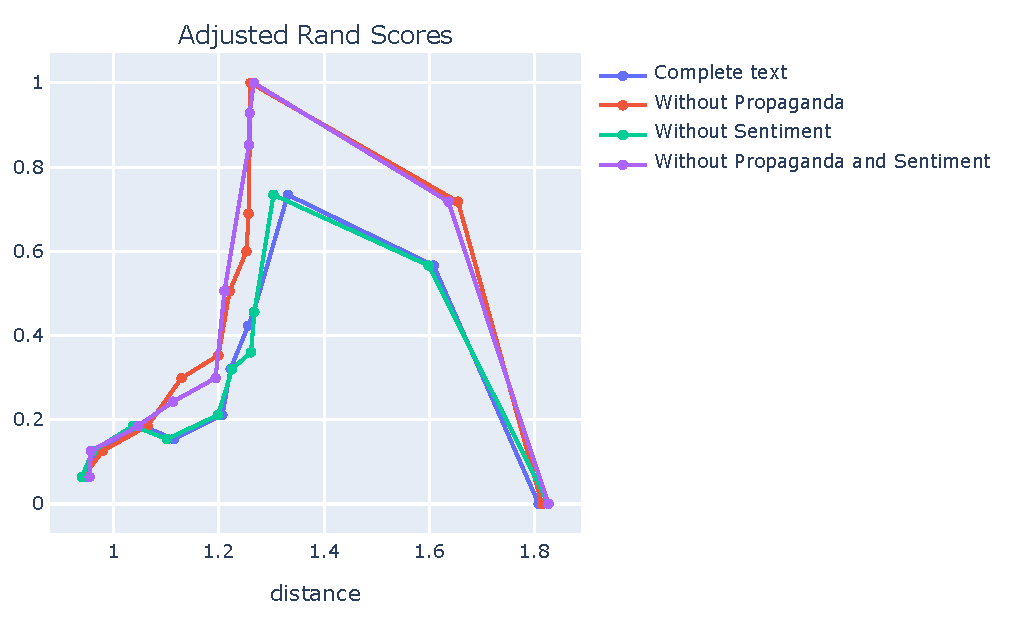
\includegraphics[width=\linewidth]{figures/sentpropnoise_4_en_tfidf_fitness_topic-cropped.pdf}
    \caption{Adjusted Rand Index on a simplified scenario (only 4 clusters to identify) using Hierarchical Agglomerative Clustering on TF-IDF features. On the $x$ axis, we have the euclidean distance which corresponds to the current progress of clustering: from the left to the right, initial small clusters are merged and become bigger.}
    \label{fig:hierarchical_sentpropnoise_evolution}
\end{figure}

% The interpretation of this curve is that, when the hierarchical clustering begins to raise the threshold, the clusters match more with the gold clusters, until a certain point where distinct clusters are merging together and therefore lowering the scores.
At this point we do the comparison with the other collections of articles where each one of them has been cleaned from sentiment and/or propaganda words. We see in this figure that, while sentiment does not look to have much impact on clustering, removing propaganda increases the ability to cluster more similarly to the reference. 

% We can compare the behaviour of this curve between the full text and the text without the loaded/propaganda pieces.
The comparison can be at the maximum point, where the threshold is optimal, % (we should truncate the clustering there)
or we can compare the full curve. For simplicity, we compare the maximum value of the curve, that in this case is $1.0$.
%reporting also the distance where it has been reached.
Nonetheless, the full curve has analogue results, as seen in the figure above (higher maximum point, higher curve).

In Figure~\ref{fig:hierarchical_sentpropnoise_evolution} we can see that removing propaganda helps TF-IDF reaching 100\% perfect clustering with threshold 1.26 euclidean distance (12 articles on 3 topics: Supreme court, Elections, Coronavirus, Supreme Court). Instead without removal, TF-IDF misplaces some elements with the full text.


% table: step 5 results? Check
\subsubsection{K-Means}
For evaluating the effects with different sizes of datasets, we show here some results with K-Means.

\begin{table}[!bp]
\resizebox{\textwidth}{!}{%
\begin{tabular}{r|r|r|llll|llll}
 &  &  & \multicolumn{4}{c|}{Headlines clustering} & \multicolumn{4}{c}{Topic clustering} \\ \cline{4-11} 
\multirow{-2}{*}{\#headlines} & \multirow{-2}{*}{\# articles} & \multirow{-2}{*}{\# topics} & \multicolumn{1}{l|}{Full text} & \multicolumn{1}{l|}{No sentiment} & \multicolumn{1}{l|}{No propaganda} & \multicolumn{1}{l|}{\begin{tabular}[c]{@{}l@{}}No propaganda\\ and no sentiment\end{tabular}} & \multicolumn{1}{l|}{Full text} & \multicolumn{1}{l|}{No sentiment} & \multicolumn{1}{l|}{No propaganda} & \multicolumn{1}{l}{\begin{tabular}[c]{@{}l@{}}No propaganda\\ and no sentiment\end{tabular}} \\ \hline
2 & 6 & 2 & \multicolumn{1}{l|}{1.0} & \multicolumn{1}{l|}{1.0} & \multicolumn{1}{l|}{1.0} & 1.0 & \multicolumn{1}{l|}{1.0} & \multicolumn{1}{l|}{1.0} & \multicolumn{1}{l|}{1.0} & 1.0 \\ \hline
4 & 12 & 3 & \multicolumn{1}{l|}{\begin{tabular}[c]{@{}l@{}}.390R\\ .553M\end{tabular}} & \multicolumn{1}{l|}{\begin{tabular}[c]{@{}l@{}}.390R\\ .553M\end{tabular}} & \multicolumn{1}{l|}{\begin{tabular}[c]{@{}l@{}}\cellcolor{green}.645R\\ \cellcolor{green}.798M\end{tabular}} & \begin{tabular}[c]{@{}l@{}}\cellcolor{green}.645R\\ \cellcolor{green}.798M\end{tabular} & \multicolumn{1}{l|}{\begin{tabular}[c]{@{}l@{}}.734R\\ .742M\end{tabular}} & \multicolumn{1}{l|}{\begin{tabular}[c]{@{}l@{}}.734R\\ .742M\end{tabular}} & \cellcolor{green}1.0 & \cellcolor{green}1.0 \\ \hline
10 & 30 & 6 & \multicolumn{1}{l|}{\begin{tabular}[c]{@{}l@{}}.616R\\ .765M\end{tabular}} & \multicolumn{1}{l|}{\begin{tabular}[c]{@{}l@{}}.616R\\ .765M\end{tabular}} & \multicolumn{1}{l|}{\begin{tabular}[c]{@{}l@{}}\cellcolor{green}.634R\\ \cellcolor{green}.771M\end{tabular}} & \multicolumn{1}{l|}{\begin{tabular}[c]{@{}l@{}}\cellcolor{green}.634R\\ \cellcolor{green}.771M\end{tabular}} & \multicolumn{1}{l|}{\begin{tabular}[c]{@{}l@{}}.547R\\ .724M\end{tabular}} & \multicolumn{1}{l|}{\begin{tabular}[c]{@{}l@{}}.547R\\ .724M\end{tabular}} & \multicolumn{1}{l|}{\begin{tabular}[c]{@{}l@{}}\cellcolor{green}.558R\\ \cellcolor{green}.730M\end{tabular}} & \multicolumn{1}{l|}{\begin{tabular}[c]{@{}l@{}}\cellcolor{green}.558R\\ \cellcolor{green}.730M\end{tabular}} \\ \hline
100 & 300 & 35 & \multicolumn{1}{l|}{\begin{tabular}[c]{@{}l@{}}.461R\\ .585M\end{tabular}} & \multicolumn{1}{l|}{\begin{tabular}[c]{@{}l@{}}.455R\\ .584M\end{tabular}} & \multicolumn{1}{l|}{\begin{tabular}[c]{@{}l@{}}.461R\\ .581M\end{tabular}} & \begin{tabular}[c]{@{}l@{}} \cellcolor{green}.467R\\ \cellcolor{green}.599M\end{tabular} & \multicolumn{1}{l|}{\begin{tabular}[c]{@{}l@{}}.271R\\ .513M\end{tabular}} & \multicolumn{1}{l|}{\begin{tabular}[c]{@{}l@{}} \cellcolor{red}.260R\\ \cellcolor{green}.516M\end{tabular}} & \multicolumn{1}{l|}{\begin{tabular}[c]{@{}l@{}} \cellcolor{green}.274R\\ \cellcolor{green}.514M\end{tabular}} & \begin{tabular}[c]{@{}l@{}} \cellcolor{red}.263R\\ \cellcolor{green}.515M\end{tabular}
\end{tabular}%
}
\caption{Results of clustering applied to TF-IDF features with K-means. Full text is compared against \textit{no sentiment} (sentiment words have been removed), \textit{no propaganda} (propaganda words have been removed) and \textit{no sentiment and propaganda}. For each row, the values represent the ARI (denoted with \textit{R}) and AMI (denoted with \textit{M} for two different granularities: headline and topic clustering. Higher values represent predicted clusters more similar to the reference ones (improvements highlighted in green), while lower values represent more difference (deterioration shown in red). The different rows represent increasing dataset size.}
\label{tab:sentpropnoise_tfidf}
\resizebox{\textwidth}{!}{%
\begin{tabular}{r|r|r|llll|llll}
 &  &  & \multicolumn{4}{c|}{Headlines clustering} & \multicolumn{4}{c}{Topic clustering} \\ \cline{4-11} 
\multirow{-2}{*}{\#headlines} & \multirow{-2}{*}{\# articles} & \multirow{-2}{*}{\# topics} & \multicolumn{1}{l|}{Full text} & \multicolumn{1}{l|}{No sentiment} & \multicolumn{1}{l|}{No propaganda} & \multicolumn{1}{l|}{\begin{tabular}[c]{@{}l@{}}No propaganda\\ and no sentiment\end{tabular}} & \multicolumn{1}{l|}{Full text} & \multicolumn{1}{l|}{No sentiment} & \multicolumn{1}{l|}{No propaganda} & \multicolumn{1}{l}{\begin{tabular}[c]{@{}l@{}}No propaganda\\ and no sentiment\end{tabular}} \\ \hline
2 & 6 & 2 & \multicolumn{1}{l|}{1.0} & \multicolumn{1}{l|}{1.0} & \multicolumn{1}{l|}{1.0} & 1.0 & \multicolumn{1}{l|}{1.0} & \multicolumn{1}{l|}{1.0} & \multicolumn{1}{l|}{1.0} & 1.0 \\ \hline
4 & 12 & 3 & \multicolumn{1}{l|}{\begin{tabular}[c]{@{}l@{}}.287R\\ .403M\end{tabular}} & \multicolumn{1}{l|}{\begin{tabular}[c]{@{}l@{}}\cellcolor{green}.543R\\ \cellcolor{green}.641M\end{tabular}} & \multicolumn{1}{l|}{\begin{tabular}[c]{@{}l@{}}.287R\\ .403M\end{tabular}} & \multicolumn{1}{l|}{\begin{tabular}[c]{@{}l@{}}\cellcolor{green}.543R\\ \cellcolor{green}.641M\end{tabular}} & \multicolumn{1}{l|}{\begin{tabular}[c]{@{}l@{}}.566R\\ .513M\end{tabular}} & \multicolumn{1}{l|}{\begin{tabular}[c]{@{}l@{}}\cellcolor{green}.713R\\ \cellcolor{green}.750M\end{tabular}} & \multicolumn{1}{l|}{\begin{tabular}[c]{@{}l@{}}.566R\\ .513M\end{tabular}} & \multicolumn{1}{l|}{\begin{tabular}[c]{@{}l@{}}\cellcolor{green}.713R\\ \cellcolor{green}.750M\end{tabular}} \\ \hline
10 & 30 & 6 & \multicolumn{1}{l|}{\begin{tabular}[c]{@{}l@{}}.313R\\ .416M\end{tabular}} & \multicolumn{1}{l|}{\begin{tabular}[c]{@{}l@{}}\cellcolor{green}.408R\\ \cellcolor{green}.509M\end{tabular}} & \multicolumn{1}{l|}{\begin{tabular}[c]{@{}l@{}}.313R\\ .416M\end{tabular}} & \multicolumn{1}{l|}{\begin{tabular}[c]{@{}l@{}}\cellcolor{green}.343R\\ \cellcolor{green}.434M\end{tabular}} & \multicolumn{1}{l|}{\begin{tabular}[c]{@{}l@{}}.301R\\ .479M\end{tabular}} & \multicolumn{1}{l|}{\begin{tabular}[c]{@{}l@{}}\cellcolor{green}.331R\\ \cellcolor{green}.507M\end{tabular}} & \multicolumn{1}{l|}{\begin{tabular}[c]{@{}l@{}}.301R\\ .479M\end{tabular}} & \multicolumn{1}{l|}{\begin{tabular}[c]{@{}l@{}}\cellcolor{green}.436R\\ \cellcolor{green}.533M\end{tabular}} \\ \hline
100 & 300 & 35 & \multicolumn{1}{l|}{\begin{tabular}[c]{@{}l@{}}.250R\\ .362M\end{tabular}} & \multicolumn{1}{l|}{\begin{tabular}[c]{@{}l@{}}\cellcolor{red}.240R\\ \cellcolor{green}.367M\end{tabular}} & \multicolumn{1}{l|}{\begin{tabular}[c]{@{}l@{}}\cellcolor{green}.251R\\ \cellcolor{green}.372M\end{tabular}} & \begin{tabular}[c]{@{}l@{}} \cellcolor{red}.234R\\ .362M\end{tabular} & \multicolumn{1}{l|}{\begin{tabular}[c]{@{}l@{}}.185R\\ .420M\end{tabular}} & \multicolumn{1}{l|}{\begin{tabular}[c]{@{}l@{}} \cellcolor{green}.191R\\ \cellcolor{red}.408M\end{tabular}} & \multicolumn{1}{l|}{\begin{tabular}[c]{@{}l@{}} \cellcolor{green}.210R\\ \cellcolor{red}.418M\end{tabular}} & \begin{tabular}[c]{@{}l@{}} \cellcolor{green}.223R\\ \cellcolor{red}.418M\end{tabular}
\end{tabular}%
}
 \caption{Results of the clustering applied to USE features with K-Means. The explanation is the same as in Table~\ref{tab:sentpropnoise_tfidf}. The difference is that the vector representations are derived from the USE model instead of computing a TF-IDF representation of the texts.}
 \label{tab:sentpropnoise_use}
\end{table}

% analysis of results
Table~\ref{tab:sentpropnoise_tfidf} is showing how, from a small corpus to bigger corpuses, the effect of removing the persuasion words is changing.
The different rows represent the number of clusters in the gold dataset.
We can notice that in the first row (2 \#headlines), with only two headlines, the metrics are seeing that the evaluation clusters are identical to the reference clusters (score of $1.0$ both ARI and AMI).

Then in the second row (4 \#headlines, we can see that also here (as previously in Figure~\ref{fig:hierarchical_sentpropnoise_evolution}), that with topic clustering we reach $1.0$ with AMI and ARI, because we manage to match perfectly with the ground truth clusters.
This happens with the removal of propaganda, while the removal of sentiment shows no effects.
With the headline clustering instead, we still have some significant improvements (from $.390R$ to $.645R$, but we cannot reach $1.0$.

In the third row (10 headlines), we still see a similar improvement caused by the removal of propaganda. In this case, the improvement is smaller, both for headline and topic clustering.

And in the fourth row, with the biggest subset of data made of 100 headlines, we see that the effects of removing sentiment or propaganda decrease for both tasks. For the headlines clustering, only when removing both sentiment and propaganda we see an improvement with the used metrics, and the improvement is quite small (change of around $1.3\%$ ARI and $2.3\%$ AMI). For the topic clustering, the scores change only of some percentage points, and we see some degradation too on the ARI metric.

% USE table 4.2
For comparison, we compute the same metrics with the same clustering method but this time with a more complex model for document embedding (USE). This sequence model has two main differences with respect to count-based models (e.g. TF-IDF): it accounts for the order of the words, because it is a sequence model, and it can make use of synonyms because it is based on the distributional semantics (semantic similarity based on the context)~\citep{firth1957synopsis}. Since this model accounts for the sequence of words, and since we may remove words and break the semantics of the articles when cleaning from sentiment or propaganda, we need to have this comparison.

Table~\ref{tab:sentpropnoise_use} shows the results when USE is used to compute the document representations.
With respect with Table~\ref{tab:sentpropnoise_tfidf}, we can see that when we remove propaganda from the articles, we have less impact. This time, the improvement is due to the removal of the sentiment from the articles.
% when size increases
Also here, as with TF-IDF, the effects of removing persuasion decay when the dataset increases in size.

% USE meaning
The meaning of these results is that with such a complex model (USE),
propaganda removal does not help, even with a small dataset. Propaganda pieces in an article are usually more than isolated words, and are spans with a longer length. Instead, adjectives (one of the common manifestations of sentiment) are frequently isolated words. USE with respect to TF-IDF is more exposed to the sequence of words, and by inspecting the ``cleaned" articles we can see that the sentences are incomplete and cannot stand. For this reason, a simpler model like TF-IDF is being helped by the removal of propaganda, while actually for USE the sentences become broken and the clustering struggles more.

% Discrepancy between AMI and ARI
In the two tables, we see that there are some cases where the AMI and ARI metrics provide opposite direction (improvement vs degradation). In those cases, we need to keep into consideration that the two metrics come from two different theories, and also that the values do not change a lot in the affected cells.
% Therefore, moving one article from one cluster to another one, may be seen as improvement or not

\subsubsection{Inspection of the predictions}

% Why? What?
In addition to the analysis of the previous paragraphs, we want to take a closer look into the predictions, to understand better the quantitative results just described.

For simplicity, we consider the case where we have 10 headlines and we use TF-IDF (corresponding to the third row of table~\ref{tab:sentpropnoise_tfidf}). We choose the TF-IDF result because it is easier to analyse the features and see what is happening.
Let’s consider for inspection the articles belonging to two clusters (IDs given by our experimentation): cluster 0\footnote{\url{https://www.allsides.com/story/biden-leads-vote-count-trump-initiates-legal-challenges}} and cluster 7.\footnote{\url{https://www.allsides.com/story/what-watch-2020-presidential-election}}. They each include three articles, and cover the US elections of 2020. The first one was published on 5th November 2020, while the second on 3rd November 2020. So they are quite similar in the entities mentioned, but the most recent one is centred on the legal challenges initiated for the vote counts while the other headline is still pre-vote (3rd of November was the election day). This means that it is challenging for clustering to differentiate between the two ground truth clusters because a lot of terms in common exist.

\begin{table}[!htbp]
    \centering
    \begin{tabular}{c|c|c}
         & Articles from headline 0 & Articles from headline 7 \\
         \hline
        Full article & 0 0 7 & 7 0 7 \\
        Without propaganda & 0 0 7 & 7 7 7
    \end{tabular}
    \caption{Inspection of how the articles belonging to two headlines get clustered when considered in full (first row) and when propaganda is removed (second row).}
    \label{tab:sentpropnoise_inspection}
\end{table}

% In the K-Means TF-IDF they have been labelled as:
% 1, 1, 0 and 0, 1, 0 with the full text, while 1, 1, 2 and 2, 2, 2 when removing the propaganda and sentiment. The first and last article of cluster 7 are able to be grouped to the cluster 7 instead of cluster 0.

% The ground truth for cluster 0 is here https://www.allsides.com/story/trump-mounts-legal-challenges-biden-gains-ground-vote-count and for cluster 7 here https://www.allsides.com/story/what-watch-2020-presidential-election . They are both about US elections (3 November and 5 November)

% what happened
From Table~\ref{tab:sentpropnoise_inspection}, we can see that one article from the headline 7 (the middle one), in the first row is clustered together with the ones from headline 0, while when propaganda is removed, it is correctly clustered together with its companions.

% Term importance
Looking at the TF-IDF features for the articles, we see that when we consider the version without propaganda, terms like \emph{win} (win, winner, ..) are removed. These terms are in common between the two clusters and act as noise for the clustering.
In this way, the distinguishing terms of each headline are able to emerge and have more importance:
\emph{Lead} in cluster 0 (5th November), 
\emph{Patience}, \emph{legal}, \emph{wait} in cluster 7 (3 November).

The removal of these terms helps in the fine-grained differentiation of the stories.
% but may not help with coarse topic clustering
However, when there are many different headlines to identify, these removals can also be detrimental.


\subsubsection{Findings and limitations} % and limitations
\label{ssec:lp_relationship_removing_findings}
% meaning of the results

From this whole experiment, we have the overall finding that removing persuasion from news articles helps to recognise clusters, but only in specific conditions:
\begin{enumerate}
    \item the clusters have to be not too many (less than 100). Increasing the number of ground truth clusters reduces the effect of the removal;
    \item for count-based models, the improvements are better when propaganda is removed. These terms act as noise and it is better to remove them to allow the topical words to have higher weights;
    \item for language models like USE, removing propaganda can in some cases be detrimental because the sentences lose the semantics on which these models work;
    \item these findings are analogous both for Hierarchical Agglomerative Clustering and for K-means.
\end{enumerate}

% Slightly easier to cluster when sentiment and propaganda words are removed from the corpus.
% So propaganda and sentiment are acting like noise in clustering.

There are some limitations to this experiment:

\begin{enumerate}
    \item when increasing the size, the difference on the metrics used become smaller and smaller. This means that this approach does not scale well to thousands of headlines;
    \item removing terms from articles makes them incorrect grammatically. For TF-IDF encoding, this is not a problem. But for USE it becomes problem;
    \item if some words belong both to persuasion and to the topic, by removing them, it becomes more difficult to form the correct cluster. This is why non-persuasive rephrasing could be needed. (choice of terms, but still some meaning).
\todo{There exists some model that rephrase propagandistic content in non-propagandistic style. What about applying them and compare?}
\end{enumerate}

\section{\statusgreen Discussion}

Responses to the 4 RQs with contributions:

\begin{enumerate}
    \item What do writers use to persuade the reader? Different persuasion techniques: sentiment / emotion manipulation, propaganda and populism (more to denote the actors than the language itself). Answered in Section~\ref{sec:lp_techniques}.
    \item How can we automatically detect those techniques? Sentiment is detected through lexicons and sentiment treebanks. Propaganda with fine-grained models and datasets, which can also be quite unreliable (low F1 of $22.5\%$). For populism we do not have detection models, but for our initial findings it seems to be weakly correlated with propaganda. Answered also in Section~\ref{sec:lp_techniques}.
    \item How are the differences between similar articles related to a different use of persuasion techniques? In some cases they are. But in the majority of the cases, the ddifferences between the articles cannot be described in terms of differences in detected sentiment or propaganda. This is due to other types of variation: word choices/synonyms that are not the same word and do not apparently bring persuasion differences. Or also we have errors in the detection (especially sentiment) that avoid us to see the changed persuasion. Answered in Section~\ref{ssec:lp_relationship_small_variations}.
    \item Is persuasion an obstacle in recognising the events in multiple articles? Yes slightly. By removing sentiment and/or propaganda, the clustering metrics improve slightly. This improvement is small but it is a sign that the non-topical layer is acting as noise/obstacle in recognising the topical layer. This is a weak verification of our hypothesis done in Chapter~\ref{ssec:lit_layers_of_info} where we assumed that the news article are a mix between two layers of topical and non-topical words.  We answered this question in Section~\ref{ssec:lp_relationship_removing}.
\end{enumerate}

% Findings:

% \begin{itemize}
%     \item 
% \end{itemize}

Overall, this chapter highlighted how, by integrating the automated detection of persuasion in news articles, we have on one side a clearer idea on the relationship between persuasion and the variations that different news sources produce when reporting events.
On the other side, we have also a deeper understanding of the limitations of the current status of this automated detection, and the repercussions it can have when we use these methods in other tasks.
Computational detection of persuasion means is quite a recent research area, and with time and more resources (datasets and models) it will clearly improve.

\section{\statusgreen Next}
% link to next chapter
In this chapter we investigated the persuasion techniques. But we have not studied the relationship between this observed persuasion in the text and the ideals/agenda/perspective of the author/outlet. It can be really useful to understand the context around the source of an article in order to interpret its persuasion.
For this reason, the next chapter will consider perspectives and political sides. In this way we will try to understand if the persuasion of each political side is similar or which are the differences. If a different goal for the persuasion also can be observed on the persuasion itself.